\documentclass[12pt, twoside]{article}
\usepackage[francais]{babel}
\usepackage[T1]{fontenc}
\usepackage[latin1]{inputenc}
\usepackage[left=1cm, right=1cm, top=1cm, bottom=1cm]{geometry}
\usepackage{float}
\usepackage{graphicx}
\usepackage{array}
\usepackage{multirow}
\usepackage{amsmath,amssymb,mathrsfs}
\usepackage{soul}
\usepackage{textcomp}
\usepackage{eurosym}
 \usepackage{variations}
\usepackage{tabvar}


\pagestyle{empty}

\begin{document}


\section*{\center{Devoir maison 1}}



\fbox{
\begin{minipage}{18cm}
\textit{Devoir � rendre sur feuille grand format \textbf{petits
carreaux} pour le \ul{lundi 5 octobre 2009}.} 

\enskip

\textit{Remarque: Un r�sultat donn� directement sans le d�tail du calcul ne
 donnera pas de point.}
\end{minipage}
}

\subsection*{Exercice 1}

\begin{enumerate}
  \item R�tablir les signes ``$\times$'' sous-entendus.
  \item Effectuer les calculs en \ul{soulignant en vert}
 � chaque �tape le calcul en cours.   
  
\end{enumerate}

$A=100-25(5-3)+ 6\div 3$ \qquad \qquad $B=(12-5)(4+3)-26-2^3$ \qquad
 \qquad $C=9^2+3-5(4^2-6)$

\subsection*{Exercice 2}

Effectuer les calculs suivants en \ul{soulignant en vert}
 � chaque �tape le calcul en cours.
 
 \enskip
 
  
 
 $U=9 + \dfrac{13+7}{2}$ \qquad \qquad $V=4+ \dfrac{60}{2 \times 15}$ \qquad 
 \qquad $W=2 \times \dfrac{33+7}{27-7}$ \qquad \qquad $X=6 +\dfrac{7-3 \times
 2}{2 \times 5 } -2,1$
 
  \subsection*{Exercice 3}

Dans un magasin, on peut voir ces 3 �tiquettes.

\enskip

\begin{center}
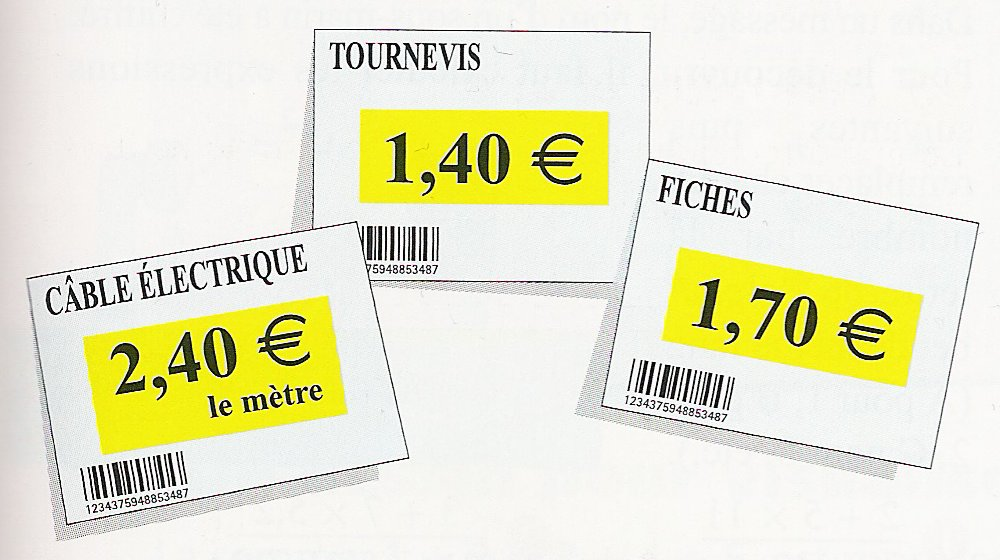
\includegraphics[width=8cm]{image/dm1_5.jpg}
\end{center}


\begin{enumerate}
  \item R�diger un texte de probl�me qui correspond au calcul $20-(7 \times
  1,40 + 2 \times 1,70 +2,40)$.
  \item Donner la solution au probl�me propos�.
\end{enumerate}

\subsection*{Exercice 4}

Pour le pique-nique qu'il va partager avec ses quatre amis, Florent ach�te 3
baguettes � 0,60 \euro \thinspace pi�ce, 2 bo�tes de thon � 1,35 \euro  pi�ce
et 500g d'emmental � 7,80 \euro  le kilo. Il paye avec un billet de 10 \euro.

\begin{enumerate}
  \item Indiquer ce qu'exprime chacun des nombres ci-dessous:
  
  $D=\dfrac{7,80}{2}$ \qquad \qquad $E=3 \times 0,60$ \qquad \qquad $F=2 \times
  1,35$
  
  $G=3 \times 0,60 + 2 \times 1,35 +\dfrac{7,80}{2}$ \qquad \qquad $H=10-\big(3
  \times 0,60 + 2 \times 1,35 +\dfrac{7,80}{2}\big)$
  \item Combien y a t-il de personnes au pique-nique? Ecrire l'expression
  permettant de calculer ce que doit payer chaque personne.
  \item Calculer le montant pay� par chacun.
\end{enumerate}
\end{document}
